\documentclass[letterpaper,9pt,twocolumn]{extarticle}
% content
\usepackage{amsmath}
\usepackage{hyperref}
\usepackage{mathtools}
\mathtoolsset{showonlyrefs}
\bibliographystyle{acm}
% layout
\usepackage[cm]{fullpage}
\usepackage{multicol}
\setlength{\columnsep}{1cm}
% spacings
\usepackage{setspace}
\onehalfspacing
\setlength{\parindent}{0pt}
\setlength{\parskip}{6pt}
\usepackage[compact]{titlesec}
% figures 
\usepackage{tikz}
\usetikzlibrary{arrows}
\usepackage{pgfplots}
\begin{document}
\twocolumn[	
	\begin{center}
		\LARGE
		\textbf{Simulation of deformation and rebound of an inflated elastic ball} 
		
		\vspace{0.5em}
		\Large
		Siyuan Chen, Xiangzhou Kong, Long Chen
	\end{center}
	\vspace{1em}
]
\section*{Abstract}
	How elasticity and interior pressure of an inflated ball or a spherical structure can be an huge impact on sports games or other aspects. Therefore, studying the model of ball bouncing can help us to predict and simulate how an elastic spherical body deforms and bounces through computational simulation. In this paper, 2-D circular structure is selected for emulating a 3-D spherical shell. Discrete elastic rods methods are applied for the simulation. For the simulation part, we used DER code in Python as well as NumPy for carrying out linear algebra. Furthermore, mass-modification method is applied for comparing with standard DER method. Compared to simple predictor-corrector method, mass-modification method is neater and it can be applied to sloped surfaces. A ``rolling ribbon'' model \cite{Raux10} is also simulated,. Finally, a variable inflation pressure model is animated to show a more realistic result. 3-D shell and collision detection simulation was attempted but we gave up due to the limited time and difficulty of debugging. 
\section{Background}
	The elasticity and pressure of an inflated ball have an impact on the sports games or other aspects. For example, the difficulty to catch a football passed by a quarterback; the distance a soccer ball can fly when kicked; the exact amount of force should be applied when a point guard is trying to make a bounce pass, etc. 
	
	Studying the model of ball bouncing can help us to predict and simulate how a elastic spherical body deforms and bounces through computing and simulation. A theoretical model for spherical ball bouncing has been established by Stronge \cite{Stronge06}, with the assumption that ball shells are thin and the internal gas pressure is high enough such that the reaction due to shell bending is insignificant in comparison with the gas pressure. 
	
	On the other hand, the FEM analysis of Bao \cite{Bao15}, neglecting the internal gas pressure, only considered the bending of the shell when the ball gets stiffer. 
\section{Potential impact}
	With discrete simulation methods, it is possible for us to take both gas pressure and shell bending into consideration. Moreover, factors like friction with the ground, other reaction forces from the ground, damping and aerodynamic drag can be included in our simulation. 

 We utilized discrete elastic rod model for 2D analysis and simulation in phase 1 of this project. 3D discrete shell model will be utilized in phase 2 of this project. While the detailed methodology will be explained in the following section, this project including the algorithm can be a prototype of analysis and simulation of objects in reality with complex geometry. Also, the simulation of the mechanical behavior of flexible structures including elastic objects such as basketballs, tires or inelastic objects such as aluminum cans or hats can be applied to animation and computer-generated imagery in movies \cite{Grinspun08}.
\section{Methodology}
	In current stage, we are using a 2-D circular structure to emulate a 3-D spherical shell. Discrete elastic rods \cite{Bergou08} methods are used for our simulation.	

	\subsection{Time marching scheme without using mass-modification method}
		Backward Euler method is used to march $\underline x$ starting from the initial position.
		\subsubsection{Discrete rod formulation}
			From Newton's second law, $ F_i = m_i\ddot q_i$, we develop:
			\begin{align}
				f_i = m_i\frac{q_i(t_{k+1}) - q_i(t_k)}{dt^2} - m_i\frac{\dot q_i(t_k)}{dt} + \frac{\partial}{\partial q_i}(E_i^b + E_i^s) - F_i^e
			\end{align}
			where, $f_i$, the reaction force, should be $0$ for each degree of freedoms that is not constrained.
			
			In this formulation,
			\begin{itemize}
				\item $E_i^b$ is the bending energy, defined as $\frac12 EI(\phi_i - \phi_{i0})^2 / dl$. This expression is derived in class;
				\item $E_i^s$ is the stretching energy, defined as $\frac12 EA \epsilon_i^2 / dl$. This expression is derived in class;
				\item $F_i^e$ is the external force, which will be discussed in later sections.
			\end{itemize}
		\subsubsection{Newton-Raphson iteration}
			We use Newton-Raphson iteration to solve each time step:
			\begin{align}
				\underline q := \underline q - \underline{\underline J} / \underline{f}
			\end{align}
			where, $J$, the Jacobian, is calculated by $J_{ij} = \frac{\partial f_i}{\partial q_j}$. The Jacobian is composed by the Hessian matrices of elastic energies in each section of the structure, and the Jacobian of different external forces that may depends on $\underline x$.
			
			The Jacobian is pre-computed with computer algebra system, leaving scalar parameters to be specified at run-time.
	\subsection{Surface contact without using mass-modification method}
		Without using mass-modification method, a simple predictor-corrector method is used to handle ground surface contact (which will be horizontal surface).
		
		Assume a ground surface at $y = 0$, When doing time-marching, on each time step:
		\begin{enumerate}
			\item Compute $\underline q(t)$ as before;
			\item Check if there exists any $y$-direction DOF $i$ such that $q_i < 0$. If there is any, set it as a temporarily constrained DOF with $y = 0$, and recompute current time step;
			\item Check if there exists any temporarily constrained DOF, such that the normal force between the surface and the node is negative (i.e. $f_i < 0$). Remove such temporary constraint, and recompute current time step.
		\end{enumerate}
	\subsection{Mass modification method}		
		The methodology described above is still not an efficient way and has a high computational cost: the Jacobian matrix changes sizes during the iterations. What's more, the simple DER method can only simulate the contact with a horizontal ground. We need a new method to deal with the contact between the ball and a sloped ground.
		
		Mass modification method proposed by Baraff \& Witkin \cite{Baraff98} provides a more flexible way to handle surface contact. We implemented mass modification method to replace the simple predictor-corrector method above.
		
		With mass-modification method, the Jacobian matrix does not change its size, which make the computation process faster than simple predictor-corrector method. Also, we utilized this model to simulate the rebounding motion on a sloped ground.
		
		In mass-modification method, we detect DOFs to be constrained and released, with the same criteria used just as before. However, instead of enforcing their position directly, we compute ``imposed velocity change'' $\underline z$ for those DOFs to stay above contact surface.
		
		Also, in time marching, use $v_i$ instead of $x_i$, effectively doing time-discretization using:
		$$\frac{\delta v_i}{\delta t} = \frac{x_i(t_{k+1}) - x_i(t_k)}{(dt)^2} - \frac{v_i(t_k)}{dt}$$
	
		In each time step, the equation of motion is also written in $v_i$: 
		$$\Delta \underline v - (dt) \underline{\underline w}\,\underline F - \underline z = 0$$ 
		
		Inversed mass matrix $\underline{\underline w}$ is used in the formulation. It is composed by $2\times2$ component matrices $\underline{\underline w_i}$, which is $\frac1{m_i}\begin{bmatrix}1 & 0\\0 & 1\end{bmatrix}$ for unconstrained nodes, $\frac1{m_i}(\underline{\underline I} - \underline n\,\underline n^T)$ for nodes constrained in $\underline n$ direction.
		\subsubsection{Newton-Raphson iteration}
			Since we are solving for $\Delta \underline v$, in each iteration:
			$$\Delta \underline v \gets \Delta \underline v - \underline{\underline J} \textbackslash \underline f$$
			
			where $\underline f = \Delta \underline v - (dt)\underline{\underline w}\,\underline F - z$ and $\underbrace{\underline{\underline J}}_{\frac{\partial \underline F}{\partial \Delta \underline v}} = \underline{\underline I} - (dt)^2\underbrace{\underline{\underline J}^{old}}_{\frac{\partial \underline F}{\partial \underline x}}$
	\subsection{Other forces}
		External force $F_i^e = F_i^p + F_i^g + F_i^d + F_i^f$
		\begin{itemize}
			\item $F_i^p$ is discretized uniform force along rods, it is used to simulate inflation pressure effect of a 3-D ball;
			\item $F_i^g$ a constant gravity force $F_i^g = m_ig$;
			\item $F_i^d$ is damping force that may depends on $q_i$ and $\dot q_i$;
			\item $F_i^f$ is frictional force that may depends on $q_i$ and $\dot q_i$.
		\end{itemize}
		\subsubsection{Inflation pressure}
			The internal inflation pressure of the ball is emulated by adding a normal force evenly distributed on the edge of a constant magnitude per unit length $f$.
			
			Pressure force is discretized by split force on each edge equally into two halves on the endpoints, and shown in Figure \ref{pressure}.
			\begin{figure}
				\centering
				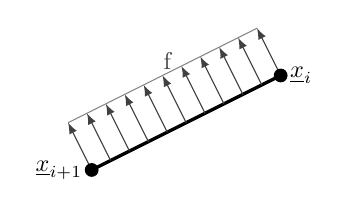
\begin{tikzpicture}[scale=0.6, every node/.style={scale=0.875}]
					\draw [very thick] (0,0) node [right] {$\underline x_i$} -- (-4,-2) node [left] {$\underline x_{i+1}$};
					\foreach \x in {0,...,10}
					\draw[darkgray,-latex,thin] (\x / 2.5 - 4,\x / 5 - 2) -- (\x / 2.5 - 4 - 0.5,\x / 5 - 2 + 1);
					\draw [gray,thin] (0 / 2.5 - 4 - 0.5,0 / 5 - 2 + 1) -- (10 / 2.5 - 4 - 0.5,10 / 5 - 2 + 1);
					\node [darkgray] at (5.5 / 2.5 - 4 - 0.6,5.5 / 5 - 2 + 1.2) {f};
					\node [circle,fill,minimum size=2mm,inner sep=0pt] at (0,0) {};
					\node [circle,fill,minimum size=2mm,inner sep=0pt] at (-4,-2) {};
				\end{tikzpicture}
				\hspace{0.1cm}
				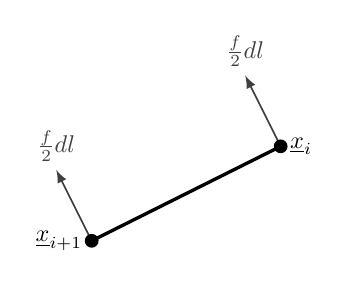
\begin{tikzpicture}[scale=0.6, every node/.style={scale=0.875}]
					\draw [very thick] (0,0) node [right] {$\underline x_i$} -- (-4,-2) node [left] {$\underline x_{i+1}$};
					\draw [darkgray,-latex,semithick] (0 / 2.5 - 4,0 / 5 - 2) -- (0 / 2.5 - 4 - 0.75,0 / 5 - 2 + 1.5) node [above] {$\frac{f}2 dl$};
					\draw [darkgray,-latex,semithick] (10 / 2.5 - 4,10 / 5 - 2) -- (10 / 2.5 - 4 - 0.75,10 / 5 - 2 + 1.5) node [above] {$\frac{f}2 dl$};
					\node [circle,fill,minimum size=2mm,inner sep=0pt] at (0,0) {};
					\node [circle,fill,minimum size=2mm,inner sep=0pt] at (-4,-2) {};
				\end{tikzpicture}
				\caption{Pressure force before and after discretization}
				\label{pressure}
			\end{figure}
		
			We also take consideration of the fact the pressure will increase when the ball is being compressed. As the ideal gas state equation says:
			$$pV = nRT$$
			If we assume the temperature is constant (which is senseful as the ambient temperature is constant as energy loss due to air compression is low), we can simple model the pressure variation with $p \propto \frac1V$. With this, the pressure at any time step is $p(t_k) = \frac{V(t_0)}{V(t_k)}p(t_k)$.
			
			The volume here is approximated by the area of the discretized structure shape, i.e. having $p(t_k) = \frac{A(t_0)}{A(t_k)}p(t_k)$. As the structure is discretized as a polygon, it is possible to use shoelace formula to calculate area:
			$$A = \frac12\left[\sum_{i=1}^{n-1}x_iy_{i+1} + x_ny_1 - \sum_{i=1}^{n-1} x_{i+1}y_i - x_1y_n\right]$$
			
			Note that, when computing the Jabobian contribution of pressure force, $J_p = \left[\frac{F_i^p}{x_j}\right]$, we neglect the pressure change due to proposed deformation. This way, local pressure force $F_i^p$ will only vary with the positions of neighboring nodes. So the Jacobian matrix is still banded. If we consider the variance in $p$, the Jacobian matrix will be dense, resulting in low linear algebraic computation speed. 
		\subsubsection{Damping}
			Damping force can be used to remove unphysical oscillations from the structure.
		
			The most simple local damping force formation would be proportional to local velocity, i.e. $F_i = -cu_i$. However, as our structure may be translating in a high bulk-velocity, such damping force is not suitable.
			
			Using a damping force proportional to velocity is a good idea to remove unphysical oscillations. To get rid of the effect of high-velocity bulk motion, we simply subtract the bulk velocity, which is represented by the velocity of the center of mass, i.e. $F_i^s = -c(u_{i} - u_{cm})$.
			
			Clearly, when the circular structure is translating with is no shape changes, no parts of the structure will receive any damping force; damping forces are only applied when deformation actually happens. Since our structure is axisymmetric, the velocity relative to the center of mass would have the same effect for different nodes. 
			
			This damping force is found effective to reduce high-frequency oscillations in our results, without slowing down the bulk motion.
		\subsubsection{Friction}
			Ideally, we expect frictional forces to follow $F_i^f = \mu f_i$, i.e. the discretized frictional force at each node is proportional to the normal force between the node and the ground surface.
			
			To reduce numerical instability and guarantee convergence, we use the following approximations:
			\begin{itemize}
				\item When calculating $F^f(t_{k+1})$, the velocity in last time step $\dot q(t_k)$ is used, instead of current velocity $\dot q(t_{k+1})$;
				\item Frictional force is reduced when velocity is very low
			\end{itemize}
	\subsection{Adaptive time stepping}
		Adaptive time stepping is a effective way to achieve stability with relatively low computational cost \cite{Soderlind06}.
		
		In previous work of \cite{Baraff98}, $\Delta x$, the proposed position change, is used as the criterion for testing whether the step size is too large. If $\Delta x$ for any point is larger than a pre-specified threshold, they discard the
		proposed state, reduce the step size, and try again.
		
		For our application, $\Delta x$ is not suitable as our bulk motion velocity is relatively high. Instead,  we experimented with different criteria for determining step sizes: velocity change $\Delta v$, contact area $A$, and reaction force $f$ are tested. It turned out that reaction force $f$ brings the best results.
		
		The reaction force per step, $fdt$, is actually the local momentum change in a time step. Once the actual $fdt$ goes above our threshold, we decrease the step size and recompute; when actual $fdt$ is below the threshold, we increase the step size. For the scale of our problems, we find a threshold of $0.005\,\mathrm{N\cdot s}$ to be appropriate.
		
		Instead of ``decrease by half, increase by double'' strategy in \cite{Baraff98},  examine the ratio of actual $fdt$ to our threshold, to determine how much do we need to increase/decrease the step size. When $fdt$ is much smaller than the threshold, we reduce step size sharper, when $fdt$ is only a little smaller than the threshold, we just reduce the step size by a little bit. Similarly, the ratio determines how large we should increase the step size by.
		
		However, instead of exactly following the ratio, we tend to be more conservative when increasing the step size, so that we can reduce the number of invalid attempts due to over-aggressive step sizes.
	
		Figure \ref{ats} shows reaction force and corresponding time step sizes used in a scene where the structure hit a surface, rebounds, and fall onto the surface again.
		\begin{figure}[ht]
			\centering
			\begin{tikzpicture}
				\begin{axis}[width=8cm,height=6cm,xlabel={$t$ [$\mathrm s$]},ylabel={$F_{max}$ [$\mathrm N$]},xmax=0.1,xticklabel style={/pgf/number format/fixed}]
					\addplot[black] table [x=t, y=f, col sep=comma, mark=none] {res/f-vs-dt.csv};
				\end{axis}
			\end{tikzpicture}\\
			\begin{tikzpicture}
				\begin{axis}[width=8cm,height=6cm,xlabel={$t$ [$\mathrm s$]},ylabel={$dt$ [$\mathrm s$]},xmax=0.1,xticklabel style={/pgf/number format/fixed}]
					\addplot[black] table [x=t, y=dt, col sep=comma, mark=none] {res/f-vs-dt.csv};
				\end{axis}
			\end{tikzpicture}\\
			\caption{Time step size versus reaction force in a typical simulation}
			\label{ats}
		\end{figure}
	\subsection{Collision between structures}
		When there are multiple structures in the simulation, it becomes necessary to have collision detection mechanisms \cite{Moore88}. As our structures are discretized circular shapes in 2-D, treating them as polygons will be sufficient.
		\subsubsection{Collision detection}
			For first implementation, we iterate though every node in the simulation, to test whether it is inside another polygon, using a point-in-polygon testing algorithm of ``crossing test'', as described in \cite{Haines94}.
			
			This can be as slow as $O(n^2)$ to number of nodes. In future, we may speed up the intersection test, by calculating the bounding box of structures, and skip collision test when the bounding box does not intersect with each other. Furthermore, we can use a quadtree to index all the nodes to enable faster collision detection.
			
			Considering our rod-like structure has a thickness, even when the centerline of two rods does not intersect, there is still a possibility that the actual structures will intersect with each other. Therefore, when a vertex of one polygon is outside another polygon (which represents the centerline), we further tests its distance to the polygon. If the distance is found to be smaller than twice the thickness, we still take it as a collision.
		\subsection{Collision reaction}
			\begin{figure}[ht]
				\centering
				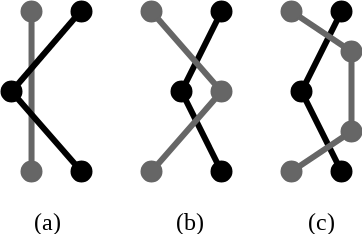
\includegraphics[width=4cm]{res/intersections.png}
				\caption{Detecting early collision}
				\label{collision-cases}
			\end{figure}
			For 2-D polygons, collision can occur in the different topologies as shown in Figure \ref{collision-cases}. In \ref{collision-cases}(a), one vertex of a polygon intrudes into one edge of another polygon. In \ref{collision-cases}(b), each polygon has a vertex intruded into another polygon, intersecting more than one edges of the intruded polygon. In \ref{collision-cases}(c), an entire edge of a polygon intrudes into another polygon.
			
			We observed that, circumstances like \ref{collision-cases}(b) and \ref{collision-cases}(c) are developed from early-stage \ref{collision-cases}(a). That is saying, when \ref{collision-cases}(b) and \ref{collision-cases}(c) are detected, we can always go back to last step, reduce the time step size and retry, and capture the early-stage collision like \ref{collision-cases}(a).
			
			With such processing, it is guaranteed we only need to process ``one point intruding into one edge'' situations.
			
			In such condition, it is possible to calculate the ``penetration depth'' $d$ of the collision, which is the depth of the vertex intruded into the edge (which might be negative) added with twice the rod thickness.
			
			With the penetration depth $d$ given, it is possible to calculate the force to be added to that intruding node:
			$$F = \frac1{dt^2}m_i d$$
			
			The direction of this force will be perpendicular to the edge being intruded. The force will be a 1st order approximation of the impulsive force needed to push the structures away from each other.
			
			For the edge being intruded, it will also experience a impulsive force of the same magnitude. This force will be distributed to the two ends of the edge. The distribution will be calculated as below:
			\begin{enumerate}
				\item Calculate the ``collision point'' on the edge, by taking the foot of the perpendicular from the intruding node to the intruded edge.
				\item Calculate the barycentric coordinate of the ``collision point'' on the edge.
				\item Distribute the collision force $F$ above (of opposite direction), to the two endpoints accordingly.
			\end{enumerate} 
		\begin{figure}[ht]
			\centering
			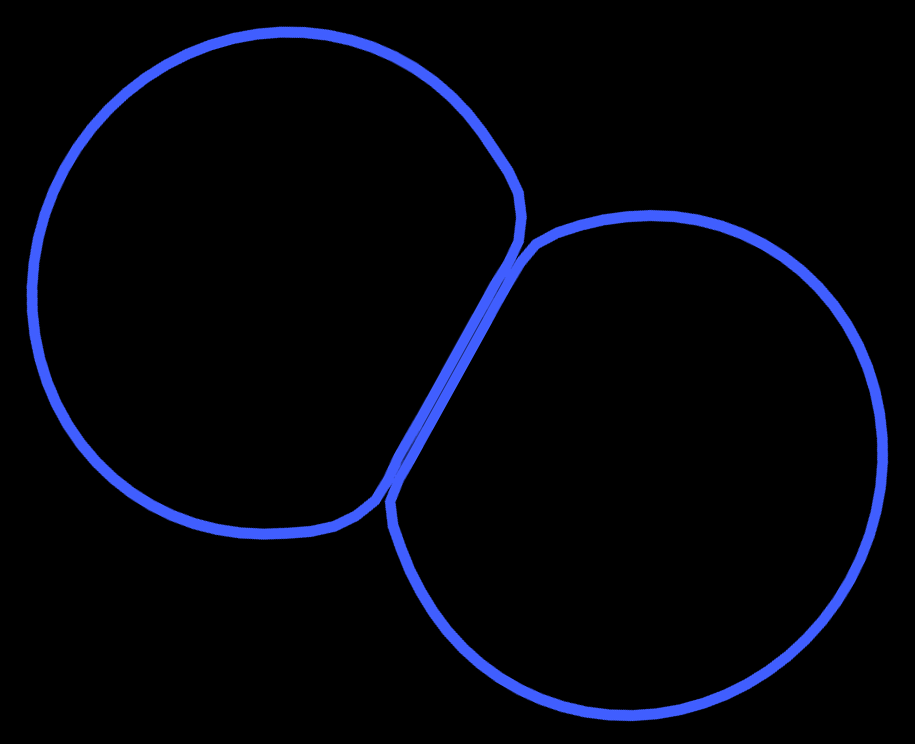
\includegraphics[width=4cm]{res/collision.png}
			\caption{Early stage of structure collision}
			\label{collision}
		\end{figure}
\section{Tools and logistics}
	Currently, we write the DER code in Python, and the library \href{http://www.numpy.org}{NumPy} is used for carrying out linear algebra. We may seek performance improvement by rewriting the code in C++ instead.
	
	The library \href{http://www.sympy.org/}{SymPy} is used for carrying out symbolic differentiation.
	
	We developed a visualization console for displaying our results, which is based on \href{https://threejs.org/}{Three.js}.	
\section{Results}
	The objectives in our project proposal is largely finished.
	
	We are able to simulate a circular structure go under deformation with our code. Pressure and damping forces are taken into account and produced physically sensible results. Surface contact with friction is taken into consideration realistically. With surface friction, the rotation while bouncing is well simulated.
	\begin{figure}[ht]
		\centering
		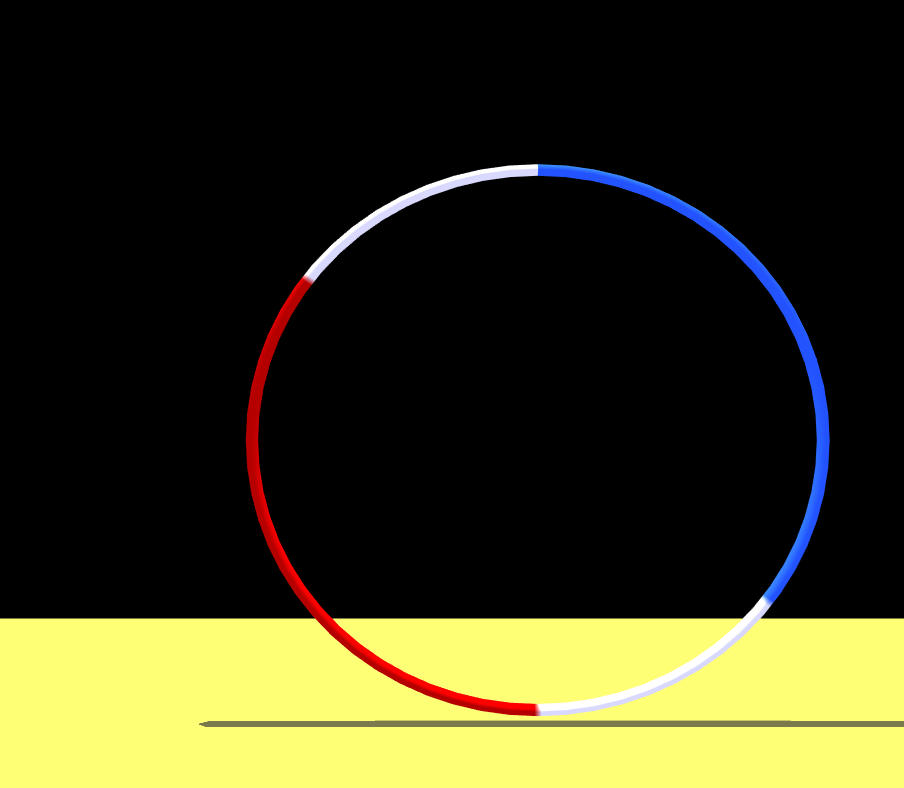
\includegraphics[width=2.75cm]{res/c-0105.png}%
		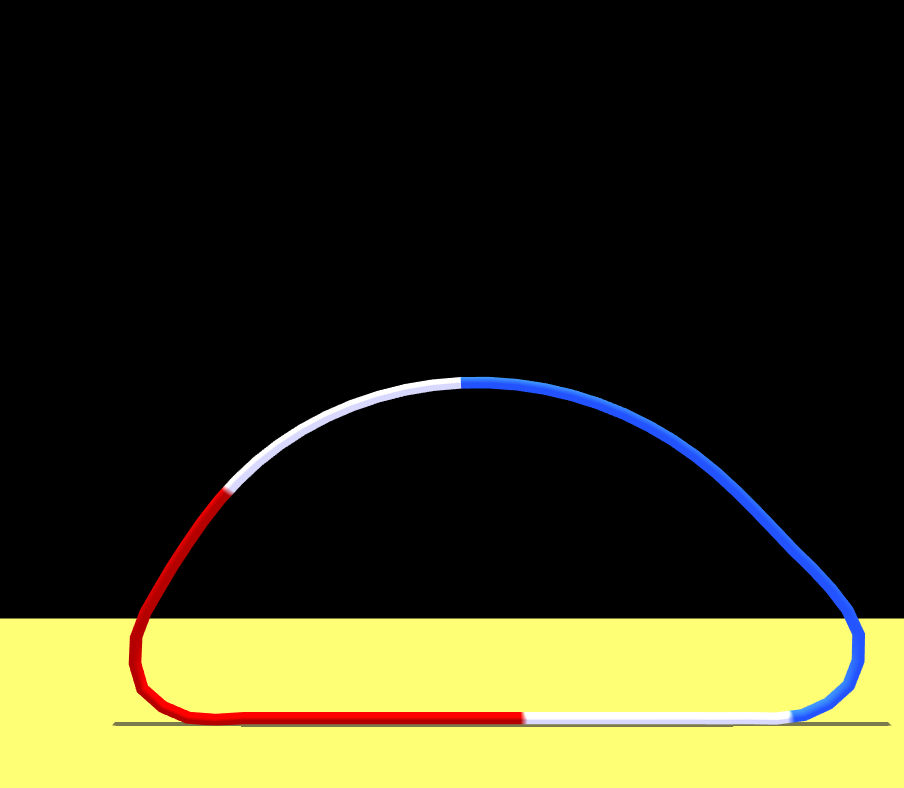
\includegraphics[width=2.75cm]{res/c-0120.png}%
		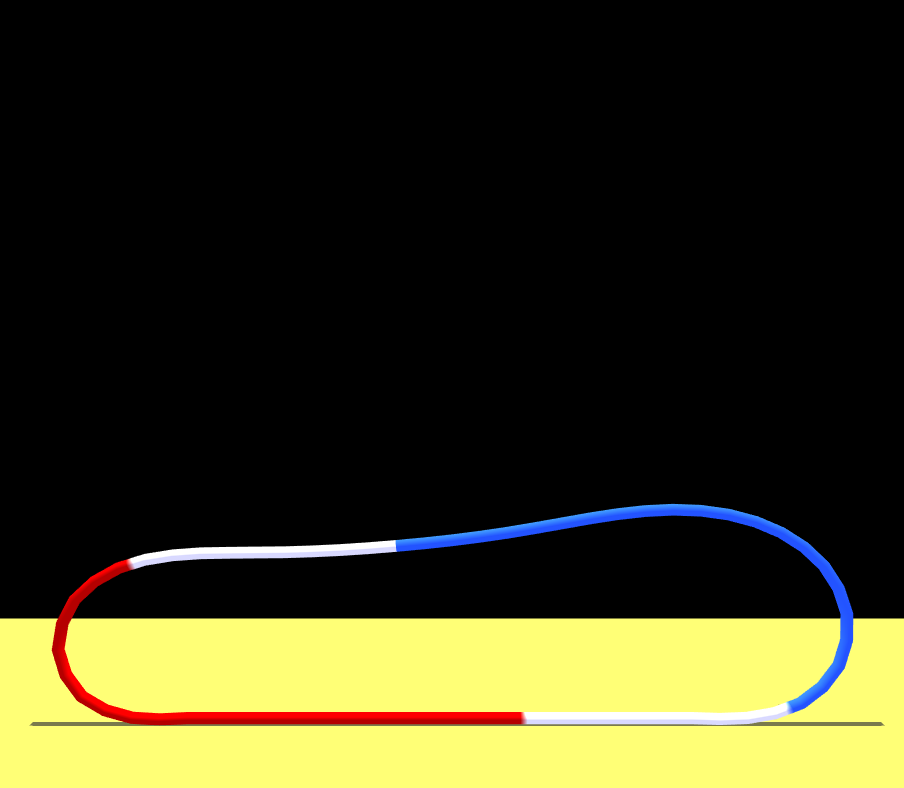
\includegraphics[width=2.75cm]{res/c-0135.png}\\
		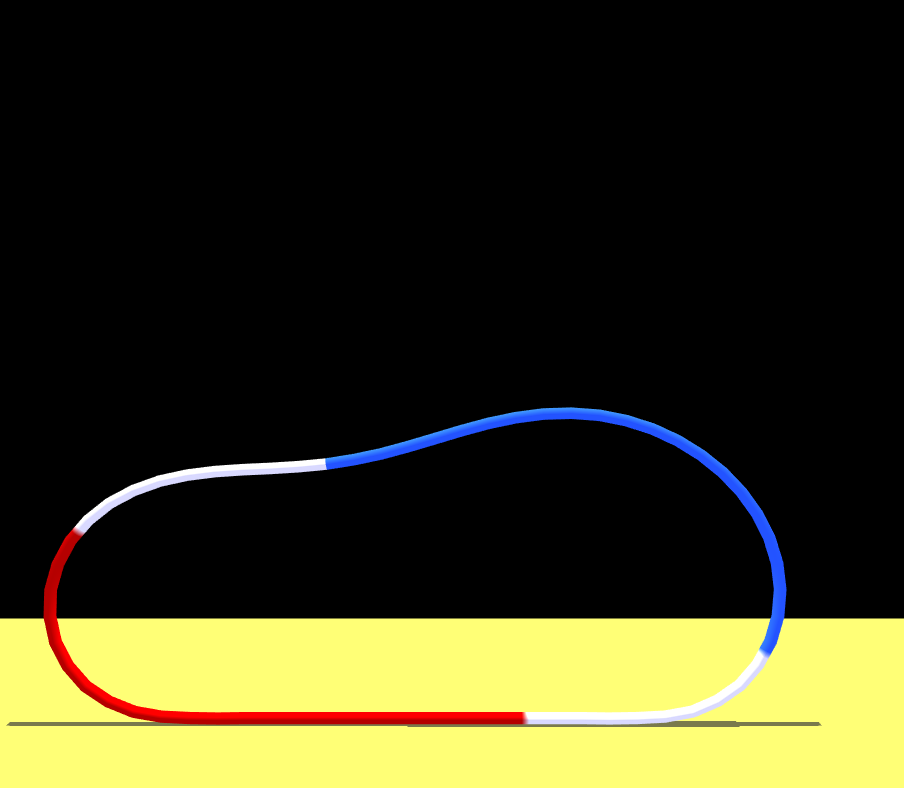
\includegraphics[width=2.75cm]{res/c-0150.png}%
		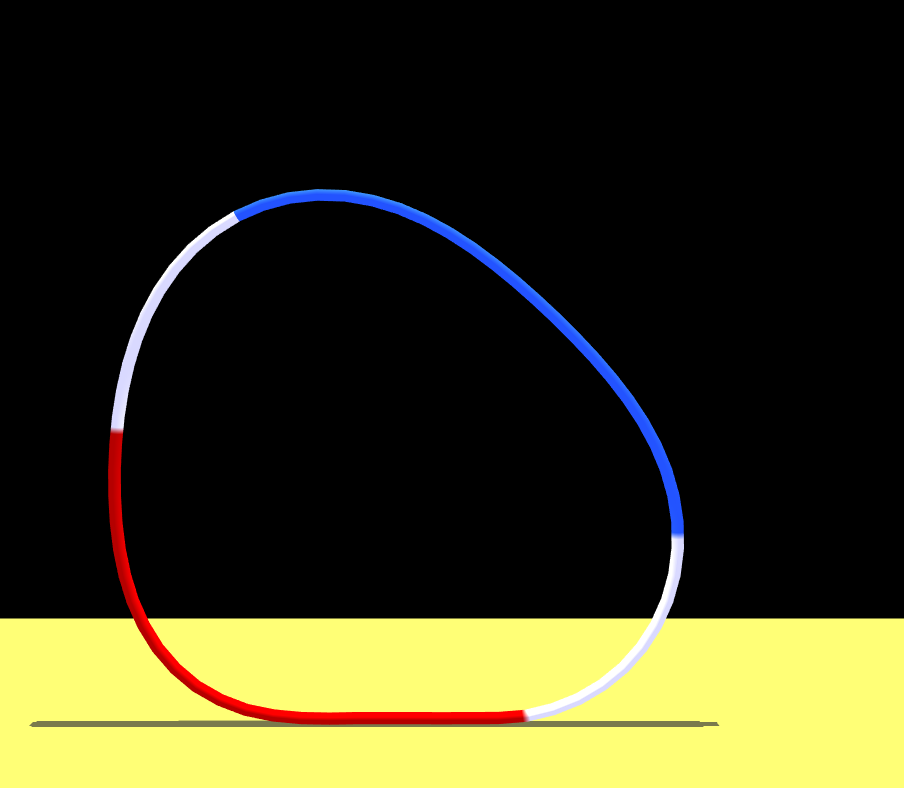
\includegraphics[width=2.75cm]{res/c-0165.png}%
		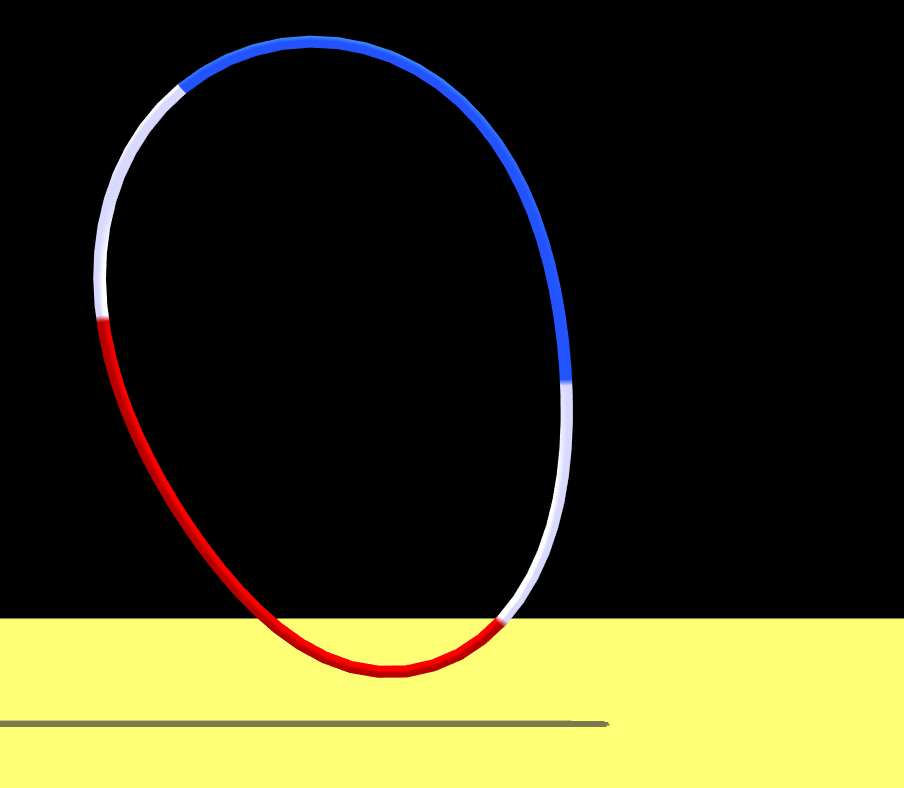
\includegraphics[width=2.75cm]{res/c-0180.png}\\
		\caption{Bounce of the structure, with $0.015\,\mathrm s$ interval}
	\end{figure}
	\subsection{Ball bouncing with different inflation pressure}
		Our assumption that a higher pressure will allow a ball to bounce better is verified by the simulation.
	
		As shown in \ref{bh}, with the same initial speed and height, a ball can bounce higher when inflation pressure in higher. Also, this effect is more significant for balls with softer surface material.
		\begin{figure}[ht]
			\centering
			\begin{tikzpicture}
				\begin{axis}[width=9.2cm,height=6cm,xlabel={$f$ [$N/m$]},ylabel={Bouncing height [$m$]},xmode=log,xticklabel style={/pgf/number format/fixed},y label style={at={(axis description cs:0.075,.5)}}]
					\addplot[black] table [x=e, y=soft, col sep=comma, mark=none] {res/bh.csv};
					\addplot[blue] table [x=e, y=hard, col sep=comma, mark=none] {res/bh.csv};
				\end{axis}
			\end{tikzpicture}
			\caption{Bouncing height with different pressure (black: $E = 10\,\mathrm{MPa}$; blue: $E = 25\,\mathrm{MPa}$)}
			\label{bh}
		\end{figure}
	\subsection{Ball deformation with different material/thickness}
		Stronge \cite{Stronge06} showed that different balls will have different deformation patterns when hitting a surface, with a figure showing that basketball will have a localized deformation, where tennis ball will deform entirely into a elliptical shape. By specifying different Young's modulus and thickness of the structure, we were able to reproduce such kind of behavior, as shown in Figure \ref{balls}.
		\begin{figure}[ht]
			\centering
			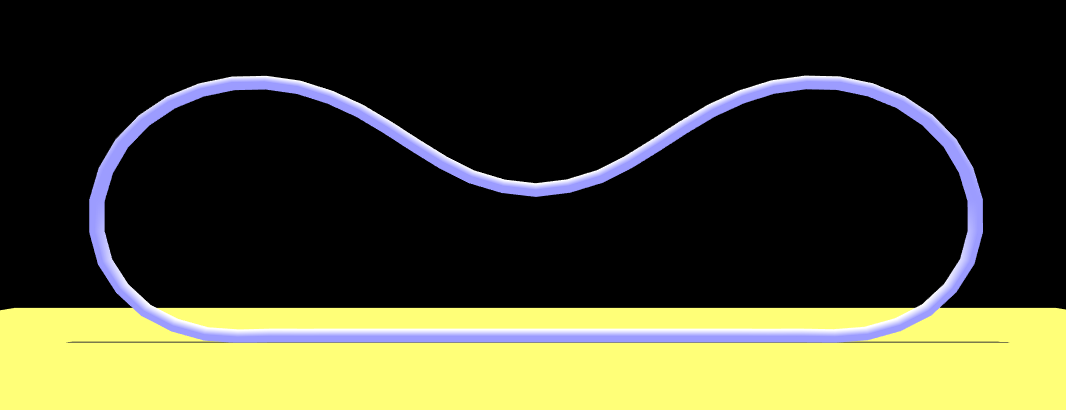
\includegraphics[height=2cm]{res/basket.png}
			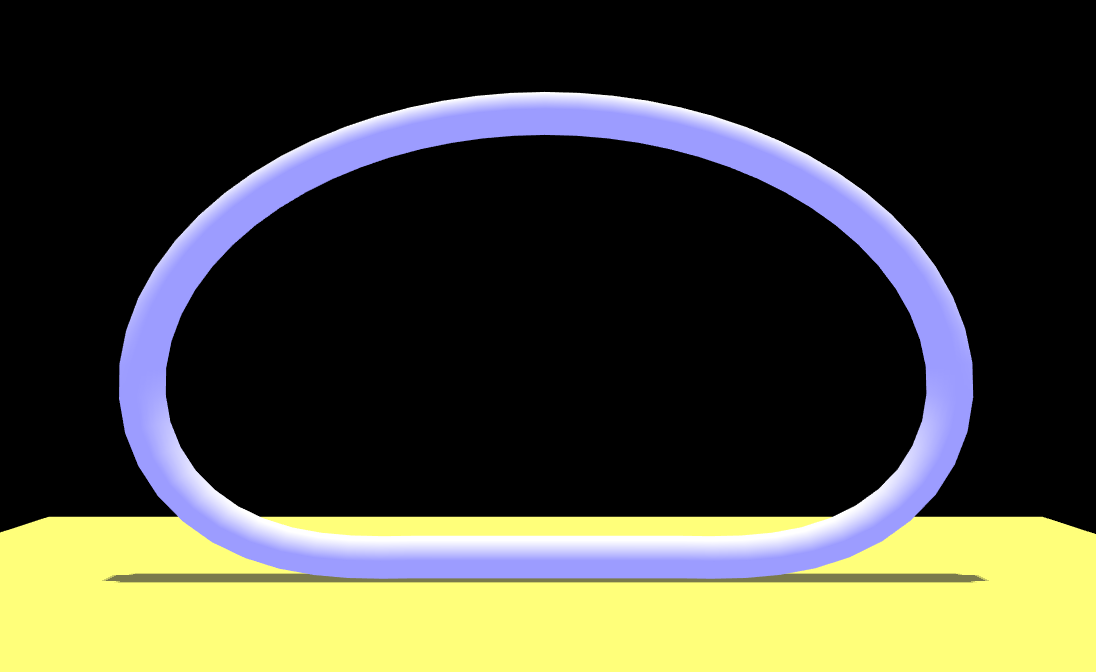
\includegraphics[height=2cm]{res/tennis.png}\\
			\caption{Deformation of different structure with same initial speed (left: basketball, right: tennis ball)}
			\label{balls}
		\end{figure}
	\subsection{Rolling}
		We created a ring model without any internal pressure, as shown in figure \ref{rr}. According to Raux \cite{Raux10}, the Normalized stiffness is directly related to Young's modulus $E$ and the aspect ratio which defined as $\frac{Height}{Diameter}$. According to Raux's theory, keeping other parameters the same, with increasing Young's modulus, the height of the rolling ribbon is increasing. The result of our simulation greatly match theirs. 
		
		\begin{figure}[ht]
			\centering
			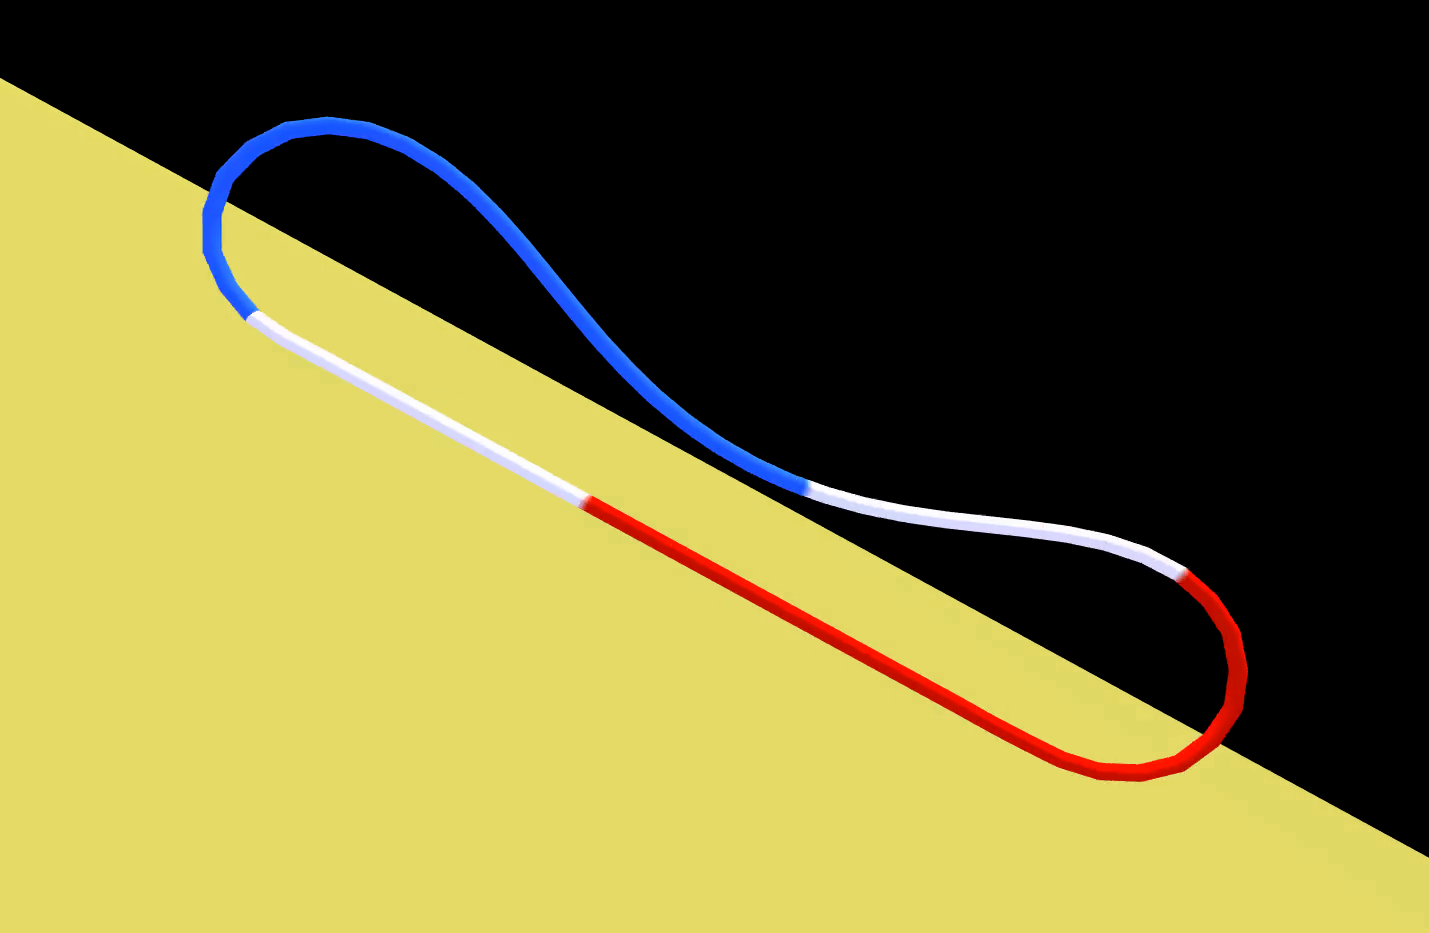
\includegraphics[width=4cm]{res/roll-2e6.png}
			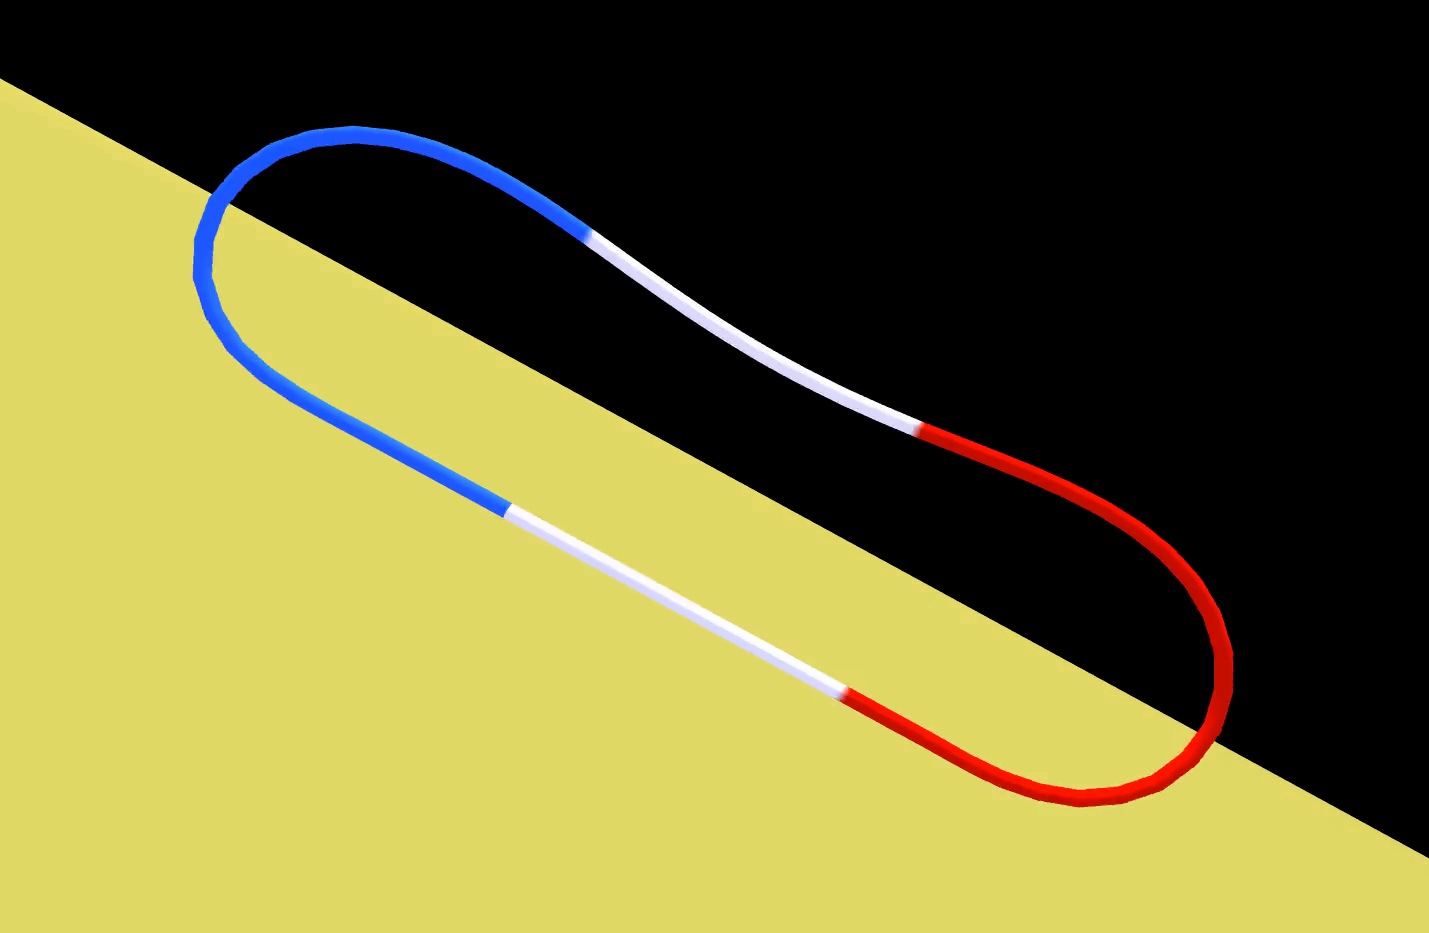
\includegraphics[width=4cm]{res/roll-3e6.png}\\
			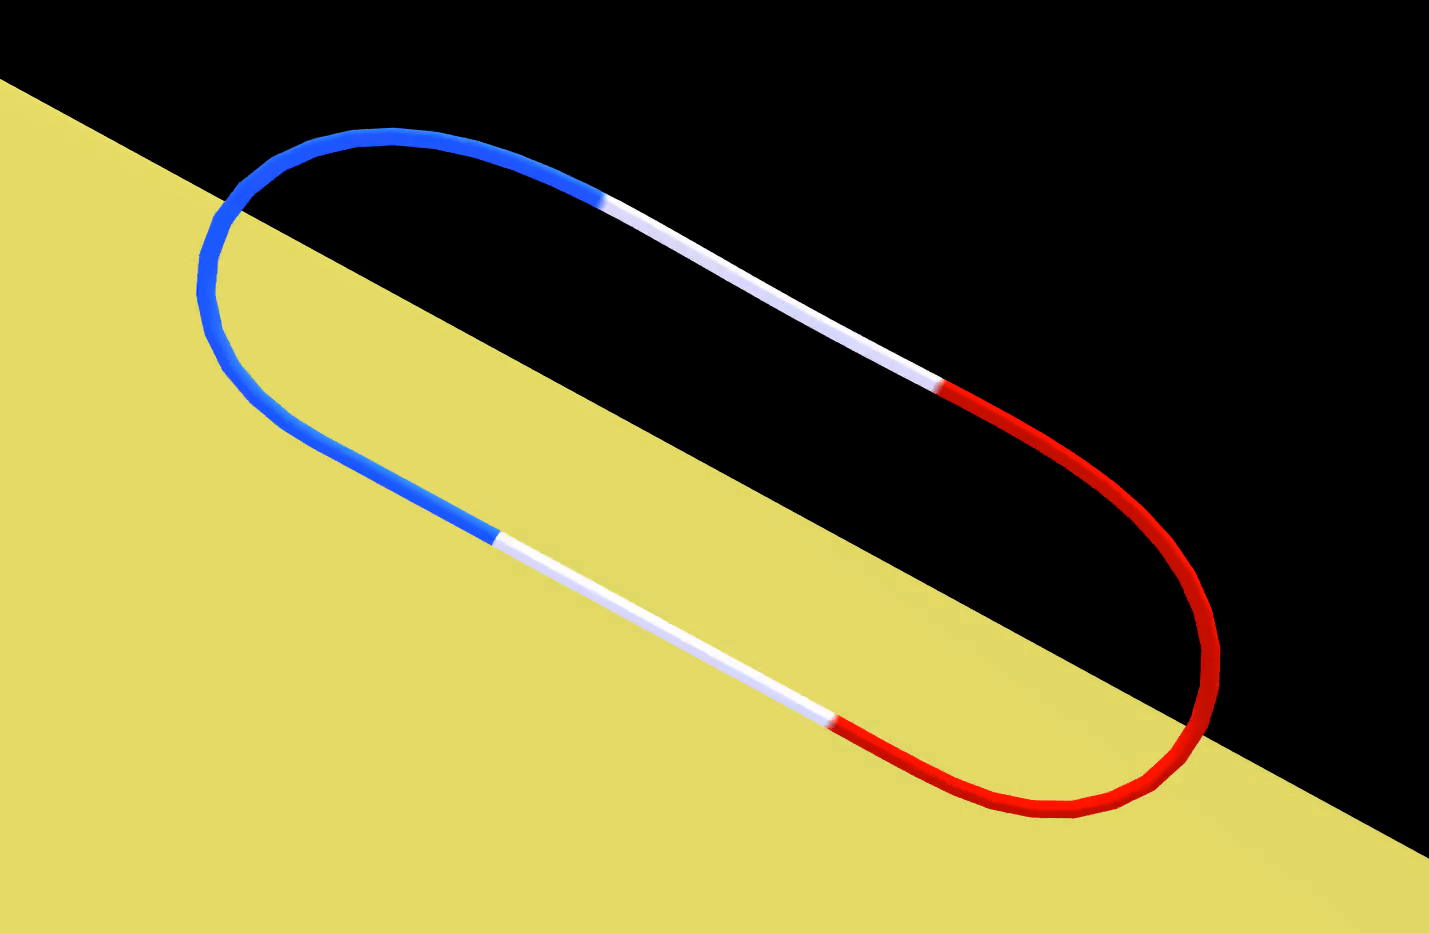
\includegraphics[width=4cm]{res/roll-4e6.png}
			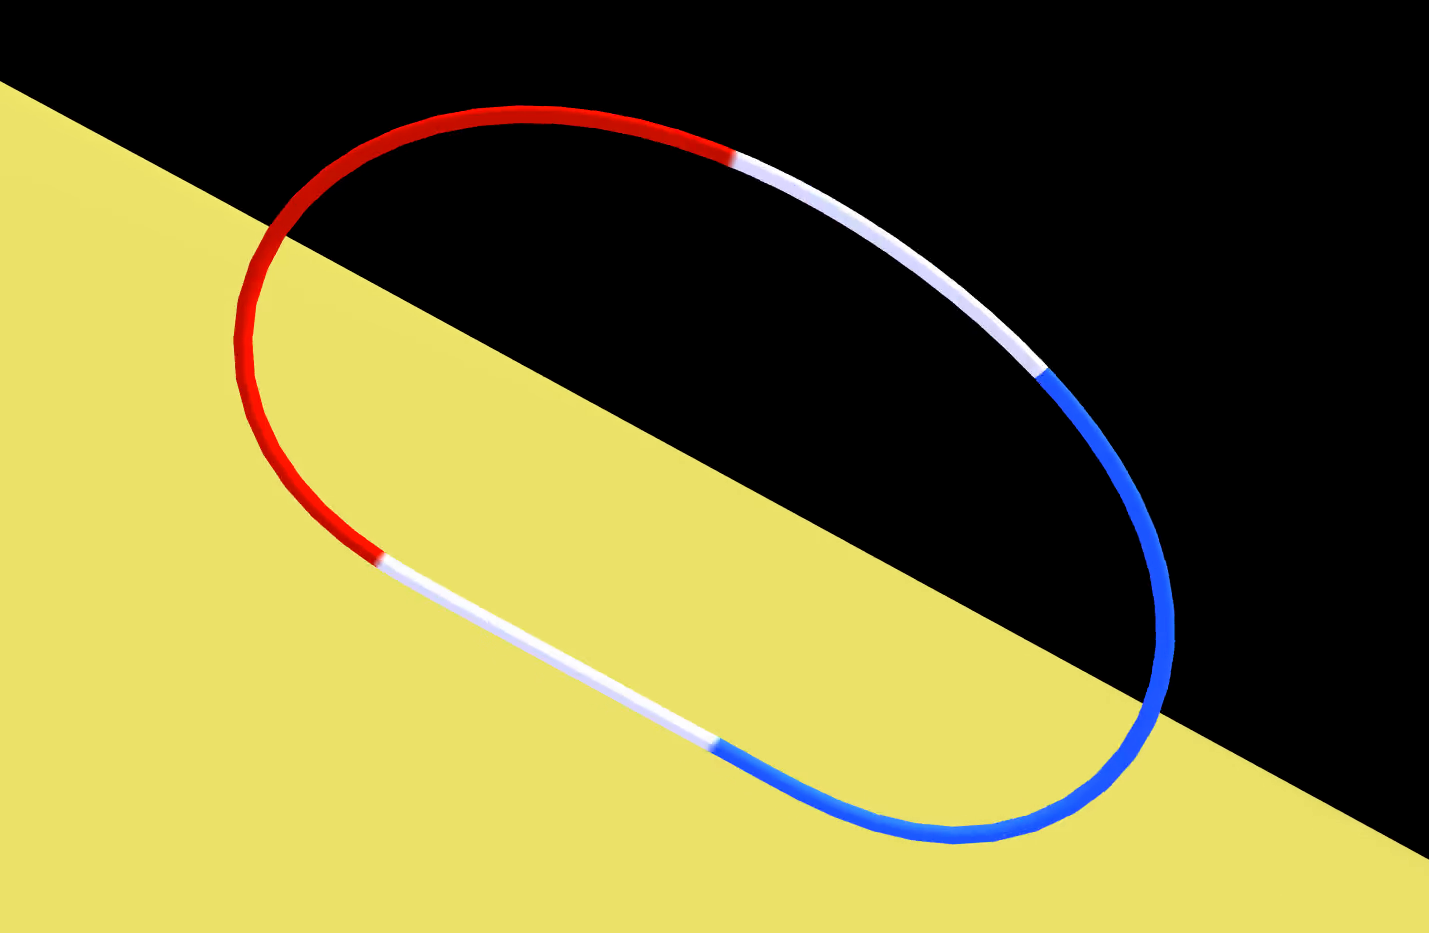
\includegraphics[width=4cm]{res/roll-8e6.png}
			\caption{Rollings rings with Young's modulus of $2\,\mathrm{MPa}$, $4\,\mathrm{MPa}$, $6\,\mathrm{MPa}$ and $8\,\mathrm{MPa}$}
			\label{rr}
		\end{figure}
		In Raux's paper, the ribbon (with same young’s modulus) was placed inside a inner surface of a drum. With fast rotating of the drum, the ribbon changes its shape alternatively. A double lobed shape appears when the velocity is increased. The reason we didn't do the velocity part is that we used gravity to accelerate the ribbon instead of giving it an changing velocity.
\section{Challenges and ongoing work}
	\subsection{3-D sphere with discrete shell}
		After finishing the 2-D scenario, we are going to apply discrete shell methods to simulate a real 3-D spherical shell in the following month.
		
		There are a few challenges:
		\begin{itemize}
			\item Generating meshes for ball that are suitable for discrete shell methods;
			\item Reducing computational time when the number of nodes are huge.
		\end{itemize}
	\subsection{Better collision detection}
		\begin{itemize}
			\item Collision detection can be more efficient, as described in corresponding sections;
			\item Self-intersection should also be detected and prevented.
		\end{itemize}
\section{Conclusion}
	By discrete elastic rod model, we can simulate the rebounding motion of a 2D circular elastic structure. Adding inner pressure inside the circular structure makes our simulation closer to a real-world 3D inflated ball case. Friction is also considered in the simulation. While dealing with the contact between the circular structure and the ground, the simulation fails and comes up with shape jittering under some specific circumstances. To fix the problem, we introduced an adaptive time step which uses smaller time step when the contact happens and uses larger time step while the circular structure is in the air in order to both accurately simulate the collision and save calculation time as much as possible.
	
	Mass-modification method is also applied to this simulation in compare with the simple DER method. The advantage of mass modification method is that the matrix size does not change during the iteration of the algorithm and saves the calculation time. Also, with mass-modification method, we can simulate the rebounding motion of the circular structure on a sloped surface. How Young's modulus affects the shape of the circular structure is also studied. Primary objective of this project, which is to simulate the rebounding motion of an inflated ball on a 2D scale, has been achieved. Further work will be done on the 3D shell model.
\bibliography{report}
\end{document}